\documentclass{beamer}
\usepackage{multicol}
\usepackage{natbib} 
\usepackage{amsmath}
\usepackage{amsfonts}
\def\newblock{\hskip .11em plus .33em minus .07em}
\newcommand\independent{\protect\mathpalette{\protect\independenT}{\perp}} 
\def\independenT#1#2{\mathrel{\rlap{$#1#2$}\mkern2mu{#1#2}}} 
\newcommand{\field}[1]{\mathbb{#1}}

%\usepackage{beamerthemeBerkeley}
% Use either the one above or the one below
\usetheme{Hannover}

\title{Regression and Causal Inference}
%\author{	F. Daniel Hidalgo\\ }
%\date{\today}

\begin{document}

\frame{\titlepage}

%\section[Outline]{}
%\frame{\tableofcontents}

\section{OLS as Prediction}

\frame{
	\frametitle{Prediction}
	
	\begin{itemize}
		\item<+-> We have an input vector $X^T = (X_1, X_2, \dots, X_p)$ with dimensions of  $n \times p$ and an output vector $Y$ with dimensions $n \times 1$. 
		\item<+-> The linear regression model has the form:
		$$ f(X) = \beta_0 + \sum_{j=1}^p X_j \beta_j $$
		\item<+-> We can pick the coefficients $\beta = (\beta_0,\beta_1,\dots,\beta_p)^T$ in a variety of ways but OLS is by far the most common, which minimizes the \textbf{residual sum of squares} (RSS):
		  \begin{align*}
			RSS(\beta) &= \sum_{i=1}^N (y_i - f(x_i))^2 \\
					   &= \sum_{i=1}^N (y_i - \beta_0 - \sum_{j=1}^P x_{ij}\beta_j)^2
			\end{align*}
	\end{itemize}
}
 
\begin{frame}[t]\frametitle{OLS in a Picture}
	
	\begin{figure}[htbp]
		\centering
			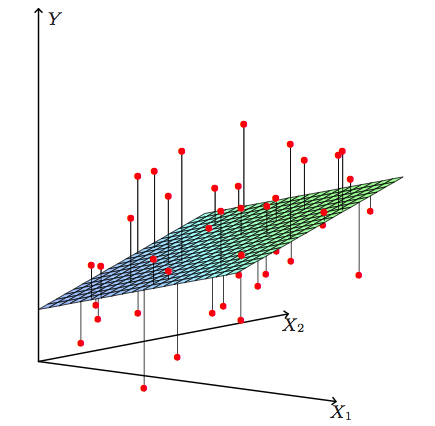
\includegraphics[height=3in]{ols.png}
		\label{fig:ols}
	\end{figure}
	
\end{frame}
 
\begin{frame}
	\frametitle{Deriving the Algorithm}
	\begin{itemize}
		\item<+-> Denote $\mathbf{X}$ the $N \times (p + 1)$ matrix with each row an input vector (with a 1 in the first position) and $\mathbf{y}$ is the output vector. 
		\item<+-> Write the RSS as:
		$$RSS(\beta) = (\mathbf{y} - \mathbf{X}\beta)^T (\mathbf{y}-\mathbf{x}\beta)$$
		\item<+-> Differentiate with respect to $\beta$:
		\begin{align}
			\frac{\partial\textrm{RSS}}{\partial \beta} &= -2 \mathbf{X}^T(\mathbf{y}-\mathbf{X}\beta)
		\end{align}
		\item<+-> Assume that $\mathbf{X}$ is full rank (no perfect collinearity among any of the independent variables) and set first derivative to 0:
		$$\mathbf{X}^T(\mathbf{y}-\mathbf{X}\beta)=0$$
		\item<+-> Solve for $\beta$:
		$$\hat \beta = (\mathbf{X}^T \mathbf{X})^{-1} \mathbf{X}^T \mathbf{y}$$
	\end{itemize}
\end{frame}

\begin{frame}[t]\frametitle{Making a Prediction}
	\begin{itemize}
		\item<+-> The \emph{hat matrix}, or \emph{projection matrix}
		\[ \mathbf{H} = \mathbf{X}(\mathbf{X}^{T}\mathbf{X})^{-1}\mathbf{X}^{T} \text{ with } \mathbf{\tilde{H}} = \mathbf{I} - \mathbf{H} \]
		\item<+-> We use the hat matrix to find the fitted values:
		 $$\mathbf{\hat{Y}} = \mathbf{X\hat{\beta}} =\mathbf{ X}(\mathbf{X}^{T}\mathbf{X})^{-1}\mathbf{X}^{T}\mathbf{Y} = \mathbf{HY}$$
		 \item<+-> We can now write
		\[ \mathbf{e} = (\mathbf{I} - \mathbf{H})\mathbf{Y}  \]
		\item<+-> If $\mathbf{HY}$ yields part of $\mathbf{Y}$ that projects into $\mathbf{X}$, this means that $\mathbf{\tilde{H}Y}$ is the part of $\mathbf{Y}$ that does not project into $\mathbf{X}$, which is the \emph{residual} part of $\mathbf{Y}$.  Therefore, $\mathbf{\tilde{H}Y}$ makes the residuals.		
	\end{itemize}
	\end{frame}
\section{Model-Based Inference}
\begin{frame}[t]\frametitle{From Algorithm to Model}
	\begin{enumerate}
	% this is the selection on observables assumption, we can't avoid it, what are we estimating if it isn't right?
	\item<+-> \emph{Linear in Parameters}: $Y$ is related to the independent variables and the error term as $Y = X\beta + \epsilon$

	% otherwise there is no variation, so we can't actually measure anything
	\item<+-> The X's are fixed and take on $\ge$ 2 values
	\item<+-> \emph{Full Rank} (in multiple regression): There is no perfect collinearity among any of the independent variables

	% otherwise x's aren't exogenous (get endogeneity bias)
	\item<+-> \emph{Zero Conditional Mean}: $E(\epsilon | X ) = 0$

	% leads to bias... but can be overcome under some assumptions about the variance matrix
	\item<+-> \emph{Homoskedasticity}: $Var(\epsilon | X) = \sigma^{2}$

	% important for the standard errors... what does it really mean to be iid and random?  Can't have autocorrelation
	% 
	\item<+-> \emph{Random Sampling}: $Y_{i}$ is an $ iid$ random sample, although this can be relaxed to $cov(y_{i}, y_{j}) = 0 = cov(\epsilon_{i}, \epsilon_{j}) \qquad i \ne j$

	% need this for our f-tests and such
	\item<+-> \emph{Normal Errors} (optional): $Y \sim \field{N}( X\beta, \sigma^2 ) $
	\end{enumerate}
\end{frame}

\begin{frame}[t]\frametitle{Deriving $\sigma^2$}
	\begin{itemize}
		\item<+-> Recall:				
			\[ \begin{array}{rrl} & \hat{\beta} &= (X^{T}X)^{-1}X^{T}Y \nonumber \\
			& &= (X^{T}X)^{-1}X^{T}(X\beta + \epsilon) \\
			\Rightarrow & \hat{\beta} - \beta &= (X^{T}X)^{-1}X^{T} \epsilon
			\end{array} \]
			\item<+-> Plugging this into the covariance equation:
			\[ \begin{array}{rl}
			cov(\hat{\beta} | X) &= E[(\hat{\beta} - \beta)(\hat{\beta} - \beta)'|X] \\
			 &= E\big[ \big((X^{T}X)^{-1}X^{T}\epsilon \big) \big((X^{T}X)^{-1}X^{T}\epsilon)' | X\big] \\
			 &= E[ (X^{T}X)^{-1}X^{T} \epsilon \epsilon^{T}X(X^{T}X)^{-1} | X] \\
			 &= (X^{T}X)^{-1}X^{T} E(\epsilon\epsilon^{T} | X) X(X^{T}X)^{-1}  \\
			 &\qquad \text{where } E(\epsilon\epsilon^{T} | X) = \sigma^{2} I_{p \times p} \\
			 &= (X^{T}X)^{-1}X^{T} \sigma^{2} I_{p \times p} X(X^{T}X)^{-1} \\
			&= \sigma^{2} (X^{T}X)^{-1}X^{T}X(X^{T}X)^{-1} \\
			&= \sigma^{2} (X^{T}X)^{-1}
			\end{array} \]
	\end{itemize}
	\end{frame}
	
	\begin{frame}[t]\frametitle{Deriving $\sigma^2$}
		We estimate $\sigma^2$ dividing the residuals squared by the degrees of freedom because the $e_{i}$ are generally smaller than the $\epsilon_{i}$ due to the fact that $\hat{\beta}$ was chosen to make the sum of square residuals as small as possible.
		\[ \hat{\sigma}^2 = \frac{1}{n-p}\sum_{i = 1}^{n} e_{i}^2 \]
	\end{frame}

\begin{frame}[t]\frametitle{Unbiasedness}
	Recall:
	%when plugging in Xbeta + epsilon, make sure to say that that is the true model...
	\begin{align*}
	 \hat{\beta} &= (X^{T}X)^{-1}X^{T}Y\\
				 &= (X^{T}X)^{-1}X^{T}(X\beta + \epsilon) \\
				 &= (X^{T}X)^{-1}X^{T}X\beta + (X^{T}X)^{-1}X^{T}\epsilon \\
				 &= \beta + (X^{T}X)^{-1}X^{T}\epsilon 
	\end{align*}
	We know that $\hat{\beta}$ is unbiased if $E (\hat{\beta}) = \beta$

	\[ \begin{array}{rl}
	E (\hat{\beta}) &= E(\beta + (X^{T}X)^{-1}X^{T}\epsilon | X) \\
	 &= E(\beta | X) + E((X^{T}X)^{-1}X^{T}\epsilon | X) \\
	 &= \beta + (X^{T}X)^{-1} E(\epsilon | X) \\
	 &\qquad \text{where } E(\epsilon | X) = E(\epsilon) = 0 \\
	E (\hat{\beta}) &= \beta 
	\end{array} \]
\end{frame}

\begin{frame}[t]\frametitle{Regression Anatomy}
	\begin{itemize}
		\item<+-> In the simple bivariate case:
		 $$\beta_1=\frac{\textrm{Cov}(Y_i,X_i)}{\textrm{Var}(X_i)}$$
		 \item<+-> In the multivariate case, $\beta_j$ is:
		$$\beta_j=\frac{\textrm{Cov}(Y_i,\tilde{X}_{ij})}{\textrm{Var}(\tilde{X}_{ij})}$$
		where $\tilde{X}_{ij}$ is the residual from the regression of $X_{ij}$ on all other covariates.
		\item<+-> The multiple regression coefficient $\hat \beta_j$ represents the additional contribution of $x_j$ on $y$, after $x_j$ has been adjusted for $x_o, x_1, \dots, x_{j-1}, x_{j+1}, \dots, x_p$ 
		\item<+-> What happens when $x_j$ is highly correlated with some of the other $x_k$'s?
	\end{itemize}
\end{frame}
\section{Regression and Causation}
\begin{frame}[t]\frametitle{Regression in  Causal Analysis}
	\begin{itemize}
		\item Imagine we are analyzing a \emph{randomized} experiment with a regression using the following model:
		$$Y_i=\alpha + \beta_1 \cdot T_i + \mathbf{X}^T_i\cdot \mathbf{\beta}_2+\epsilon_i$$
		where $T_i$ is an indicator variable for treatment status and $\mathbf{X}_i$ is a vector of \emph{pre-treatment characteristics}
		\item<+-> Under this model, what is random?  
		\item<+-> How do we interpret the coefficients on $\mathbf{X}_i$?
		\item<+-> How do we interpret the coefficient  $\beta_1$? 
		
	\end{itemize}
\end{frame}

\begin{frame}[t]\frametitle{Regression in an Observational Study}
	\begin{figure}[htbp]
		\centering
			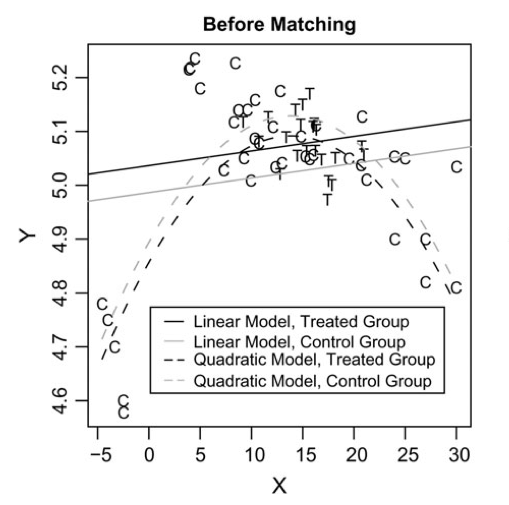
\includegraphics[height=3in]{model_dependence.png}
		\caption{caption}
		\label{fig:model_dependence}
	\end{figure}
	
\end{frame}

\end{document}
